\documentclass[preprint,3p,onecolumn]{elsarticle}

\usepackage{lineno,hyperref}
\usepackage{natbib}
\usepackage{lipsum}
\usepackage{float}

\modulolinenumbers[5]

\journal{Journal of Kybernetes}

\usepackage{natbib}
\bibliographystyle{abbrvnat}
\setcitestyle{authoryear,open={(},close={)}}
\graphicspath{{./figures}}
\usepackage{lineno}


\begin{document}
\begin{frontmatter}

\title{Optimization of purchasing business process in Moroccan public universities based on COBIT and artificial intelligence techniques}

% \author{Sakyoud Zakaria, Aaroud Abdessadek, Akodadi khalid}
% \address{Chouaib Doukkali University}
% \address{Faculty of Sciences of El Jadida}

\begin{abstract}
The Moroccan Court of Accounts often highlights that the purchasing business process in the public sector in general and public universities is a budgetary loophole. In this research work, we propose a new approach to the organization and execution of the purchasing business process in Moroccan public universities. Our approach aims to establish a system of transparency and governance best practices to minimize both financial and temporal waste. The proposed approach enhances the actual purchasing business process with control objectives for information and related technology, the COBIT 2019 guidelines, and artificial intelligence techniques. COBIT 2019 aligns the purchasing business process with conventional regulations and best practices in IT governance. Based on these guidelines, an intelligent recommendation system is proposed to generate an optimal purchasing order and overcome the limitations of this business process. The intelligent recommendation system is experimented on in the purchasing of IT products (hardware, gear, etc.) in our faculty. Experimental results demonstrate that our approach contributes to limiting financial and time wastage and promotes transparency in this business process.
\end{abstract}

\begin{keyword}
\texttt{Business process optimization}\sep purchasing business process \sep COBIT 2019 \sep artificial intelligence
\end{keyword}

\end{frontmatter}

\section{Introduction}

\par Owing to the COVID-19 pandemic, the World Bank estimated that most major economies will lose at least 2.5 percent of their gross domestic product (GDP) value \citep{world2020global}. In developing countries like Morocco, the impact may be even more prominent, and the government will inevitably find loans to overcome the economic damage. This necessarily implies an increase in external debt, which places the country in a vicious circle that delays economic development. To limit external borrowing, the government must optimize internal expenses and optimally limit waste linked to bad governance. Our current research fits this endeavor. We propose a new approach to the organization and execution of the purchasing business process  at Moroccan public universities. In fact, the Moroccan Court of Accounts often highlights the purchasing business process in the public sector in general and public universities, particularly as a budgetary loophole. Thus, the proposed approach aims to establish a system of transparency and governance best practices in this business process.
\par Our proposed approach enhances the actual purchasing business process with Control Objectives for Information and Related Technology (COBIT) 2019 guidelines and artificial intelligence techniques. COBIT 2019 aims to align purchasing business process with conventional regulations and best practices in IT governance. Artificial intelligence techniques are used to establish an intelligent recommendation system. This recommendation system takes purchasing preferences as technical features as input and then executes a series of filters on local and crawled data to propose suitable products in quality and cost. Hence, the final output of the recommendation system is the optimal purchasing order. Actual state regulations on purchasing business processes stipulate that the optimal purchasing order is chosen according to lowest bidder principal. This approach does not guarantee compliance with average market costs. Purchasing order can be excessive, despite proposing lowest price. Hence, the proposed recommendation system proposes an alternate approach that defines optimal purchasing order based on utility theory \citep{fishburn1968utility}.
    
\par The intelligent recommendation system is experimented on the purchasing of IT products and gears, and the purchasing scenario is established in our computer science department. Experimental results demonstrated that our approach contributes to limiting financial and time waste and promotes more transparency in the purchasing business process.

\par We aim to answer the following key research question: How can we promote transparency, limit financial wastes, and reduces execution time in the purchasing business process of Moroccan public universities? To gather the answers, we first studied the current purchasing business process. This process is then formalized to analyze and highlight its weaknesses. This analysis enabled us to approach the “to-be” purchasing business process. We then propose a recommendation system that constitutes an execution framework for this business process. We have conceived this recommendation system as an organizational tool and as a vector to governance best prices to answer the previous research question.

\par The paper is structured as follows:

\begin{itemize}
\item Section 2 presents the research methodology.
\item Section 3 discusses related works and contributions and positions the current paper.
\item Section 4 presents and models the purchasing business process in Moroccan public universities.
\item Section 5 overviews the motivation scenario and the theoretical background of our proposition
\item Section 6 presents the intelligent recommendation system and its components and workflow
\item Section 7 presents the implementation of the intelligent recommendation system.  A prototype is developed and tested on a real purchasing use case in computer science department.
\item Section 8 discusses the results
\item Section 9 anticipates the perspectives of our future works 
\end{itemize}

\section{Research methodology}
\par In this paper, we followed the design science research (DSR) methodology for information systems \citep{peffers2012design}. Design science research is a research paradigm wherein a designer answers questions relevant to human problems through the creation of innovative artifacts, thereby contributing new knowledge to the body of scientific evidence. These designed artifacts are both useful and fundamental for understanding research problems \citep{hevner2010design}. Correspondingly, this research aims to provide an artificial intelligence-based system and a set of COBIT 2019 guidelines to optimize the purchasing business process in Moroccan public universities. The DSR implementation in this study ( figure \ref{rdm}) was inspired by \citep{peffers2007design} \citep{hevner2010design} \citep{hevner2004design} \citep{hevner2004design}. This implementation comprises six steps.
\begin{enumerate}
\item Problem identification and motivation: Problem identification is principally the analysis of the current purchasing business process to highlight zones of inefficiency. A motivation scenario is also presented to express the motivations behind our proposition.
\item Definition of the objectives for a solution: The main objective is the optimization of the purchasing business process from an organizational perspective and also to construct an AI-based recommendation system to support an efficient and transparent execution of the purchasing business process.
\item Design and development: The analysis, design and technological choices for the development of the recommendation system are presented in Section 4 and Section 5. Fundamentally, we have adopted an agile methodology \citep{ highsmith2002agile} all over the design and development process. Agile methodology promotes continuous iterative layers in development and testing throughout the project's life-cycle. To represent and formalize the purchasing business process, BPMN business process diagrams \citep{white2004introduction} have been used. This BPMN diagram is a conceptual contribution of this paper and fits in a larger BPMN modeling of all business process of the university.
\item Demonstration: The demonstration phase is presented in Section 7 wherein the developed recommendation system is tested. Through a real live use case. the demonstration illustrates how the recommendation system supports the purchasing business process. The use case simulates the process of purchasing computer-related material in our faculty.
\item Evaluation: The recommendation system has been evaluated and discussed regarding the initial objectifies. 
\item Communication: Research work has been communicated in the current paper.
\end{enumerate}

\begin{figure}[H]
\centering
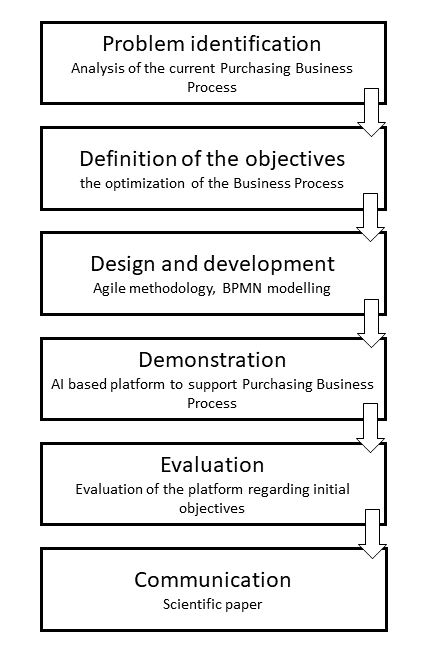
\includegraphics[scale=.5]{rdm}
\caption{Implementation of Design Science Research Methodology for Information Systems}
\label{rdm}
\end{figure}


\section{Related works}
\par We have chosen the following research works as they share with our proposal the recommendation of products to users based on initial data or metadata. We analyzed these related works based on eight axes: graphic user interface, use of review dataset, product information filtering, product review filtering, criteria ponderation, proposal of similar products, use of sentiment analysis for review classification, and finally the classification algorithm used in the sentiment analysis process. 

\par In \citep{hwangbo2018recommendation}, the authors proposed a system that extends item-based collaborative filtering algorithm. In terms of data, this system combines "online product click data" (metadata) and offline product sale data. This combination represents the customers’ online and offline preferences. These preferences were traced over time. The recommendation system aims to offer substitute and complementary products by exploring product category information based on a scoring system. This field of study focuses on fashion products, and the proposed system was adapted into this domain’s characteristics. First, preferences for fashion products appear using online click and purchase data to generate recommendations. Second, preference for fashion products decreases over time. Finally, the product that the customer wishes to purchase replaces or supplements the product that the customer prefers before.
\par Authors in \citep{bang2020product} also propose a product recommendation system. Unstructured data have the potential to be transformed into information that companies and users can employ using appropriate processing and analyses. However, existing systems do not reflect the detailed information they collect (e.g., user characteristics, purchase preferences, or purchase priorities) while analyzing review data. Therefore, providing customized recommendations to various users is challenging. Therefore, in this study, we have developed a product recommendation system that considers the user’s priority, which they select, when searching for and purchasing a product. The recommendation system then displays the results to the user by processing and analyzing their preferences. Because the user's preference is considered, the user can obtain more relevant results.

\par Research work proposed in \citep{martins2017intelligent} adheres to the emergence of data marketplaces as an alternative to traditional data commerce as they provide appropriate online environments for data offering and purchasing. Nevertheless, as the number of available purchase datasets increases, the task of buying appropriate offers is often challenging. In this sense, we propose an intelligent decision support system to help buyers purchase data offers based on multiple-criteria decision analysis. Experimental results show that our approach provides an interactive way to address buyers’ needs, allowing them to state and easily refine their preferences, without any specific order, via a series of dataset recommendations.

\par Research work in \citep{yoshikawa2019product} propose a recommendation system that suggests product alternatives. This study highlights the limitations of traditional recommendation systems that cannot recommend alternative products when existing product reviews are negative about a specific product (e.g., price, battery). Hence, this study proposes a purchasing recommendation system that focuses on review data. In fact, two types of reviews are analyzed from comments on e-commerce websites: complaint information and satisfaction information. The recommended alternative products are those that solve product complaint information. Complaint information is extracted based on product review analysis. This separation is performed by extracting negative and positive information from product reviews. Subsequently, a review analysis outputs the higher-rated products that will be used to propose alternative products by solving complaints.

The following table ( Table \ref{tableau_comparatif}) summarizes the comparison between these related works and our proposal, according to the previously mentioned axes.
\begin{table}[H]
\centering
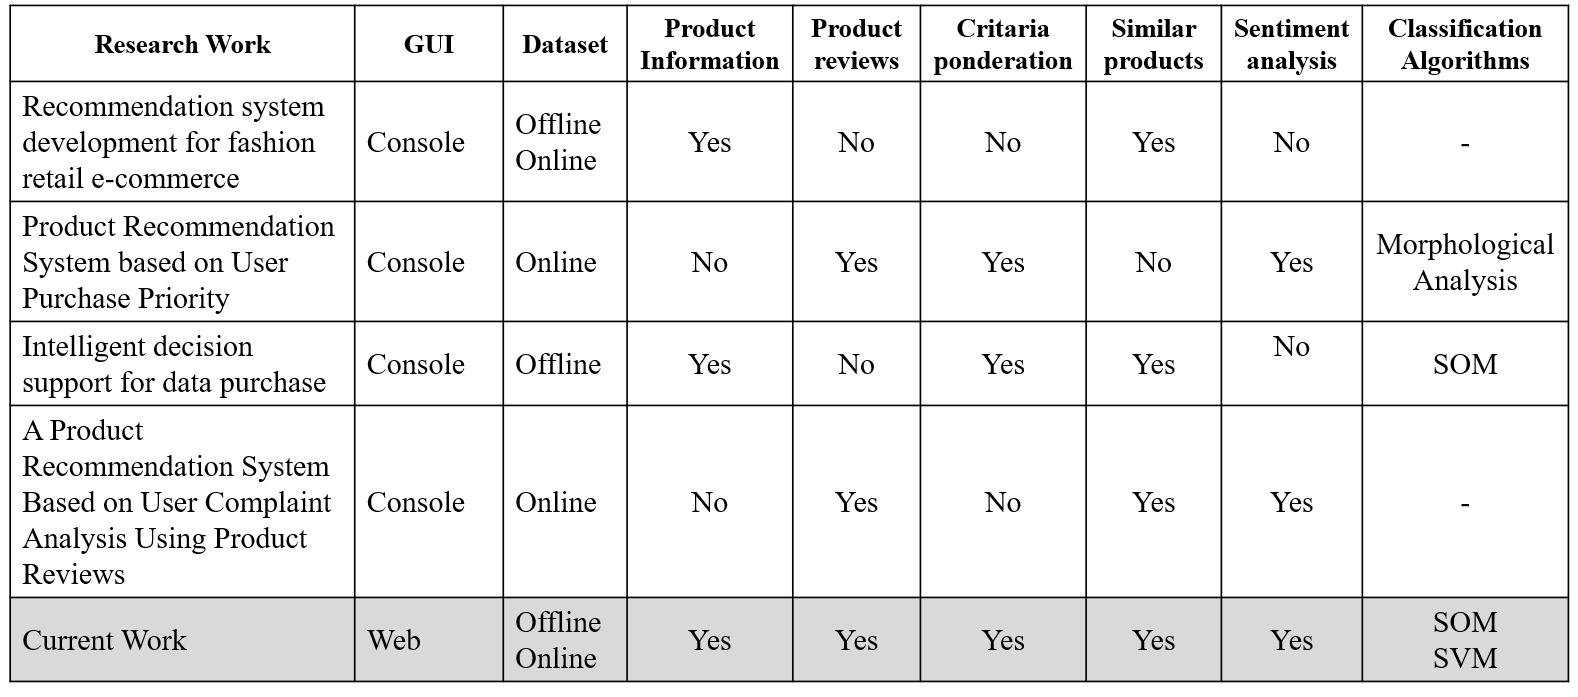
\includegraphics[scale=.4]{tableau_comparatif}
\caption{Comparative table of the related work}
\label{tableau_comparatif}
\end{table}

\section{Purchasing business process in Moroccan public universities}
\subsection{Presentation}
\par Purchasing in the public sector is quite different and more challenging compared to the private sector. In the public sector, the purchasing operation must satisfy specific state regulations and laws, and money must be spent prudently and cleverly. Therefore, purchasing services and staff are pressured to make efficient procurement decisions, and delivery time is more efficient. 
\par In Moroccan public universities, purchasing business process create and execute an obligation that entails an expense to be paid by the authorizing officer to meet the university’s needs. This process applies to all acts of engagement (markets, purchase order, contract, agreement); normative references for this process are as follows:
\begin{itemize}
\item Decree n ° 02-06-388 of the 16 Moharrem 1428 (05-02-2007) bearing the regulation of the public markets
\item Order No. 2-2471 of May 17, 2005 concerning the financial and accounting organization of universities
\item Law 69.00 on state financial control of public enterprises and other sectors
\item Dahir n ° 01-02-25 of the 03 April 2002 promulgating the law n ° 61-99 relating to the responsibility of the authorizing officers, controllers, and public accountants
\item Note 2-2471 DE / SPC of the DEPP concerning the financial and accounting organization of universities.
\item Law 21-00 on the opening date and the closing date of the accounting years of universities.
\item Decree 2-89-61 of 10 RABIA II 1410 (November 10, 1989) setting the rules applicable to the accounting of public institutions. (OO No 4023 of 6 December 1989).
\item Royal Decree No. 330-66 of 10 March 1387 (April 21, 1967) on the General Regulation of Public Accounting. (Official Bulletin No. 2843 of April 26, 1967)
\item Code of Obligations and Contracts (DOC)
\item Paying Treasurer's Guide
\item C.C.A.G.T
\item General Accounting Standards Code (CGNC)
\item C.C.A.G. MO
\end{itemize}

\subsection{BPMN modeling of the purchasing business process}
Based on previous normative references, we established the PBMN model \citep{white2004introduction} of the purchasing business process, where BPMN stands for business process model and notation. BPMN is an ISO-certified standard (ISO/IEC 19510:2013) for describing business process semantics as its notation is generally easy to comprehend and is highly understandable for business and technical personnel \citep{ritter2011building}. BPMN provides businesses and organizations with the capability to understand their internal business processes in a graphical notation to analyze and communicate these business processes in a standard manner.

\begin{figure}[H]
\centering
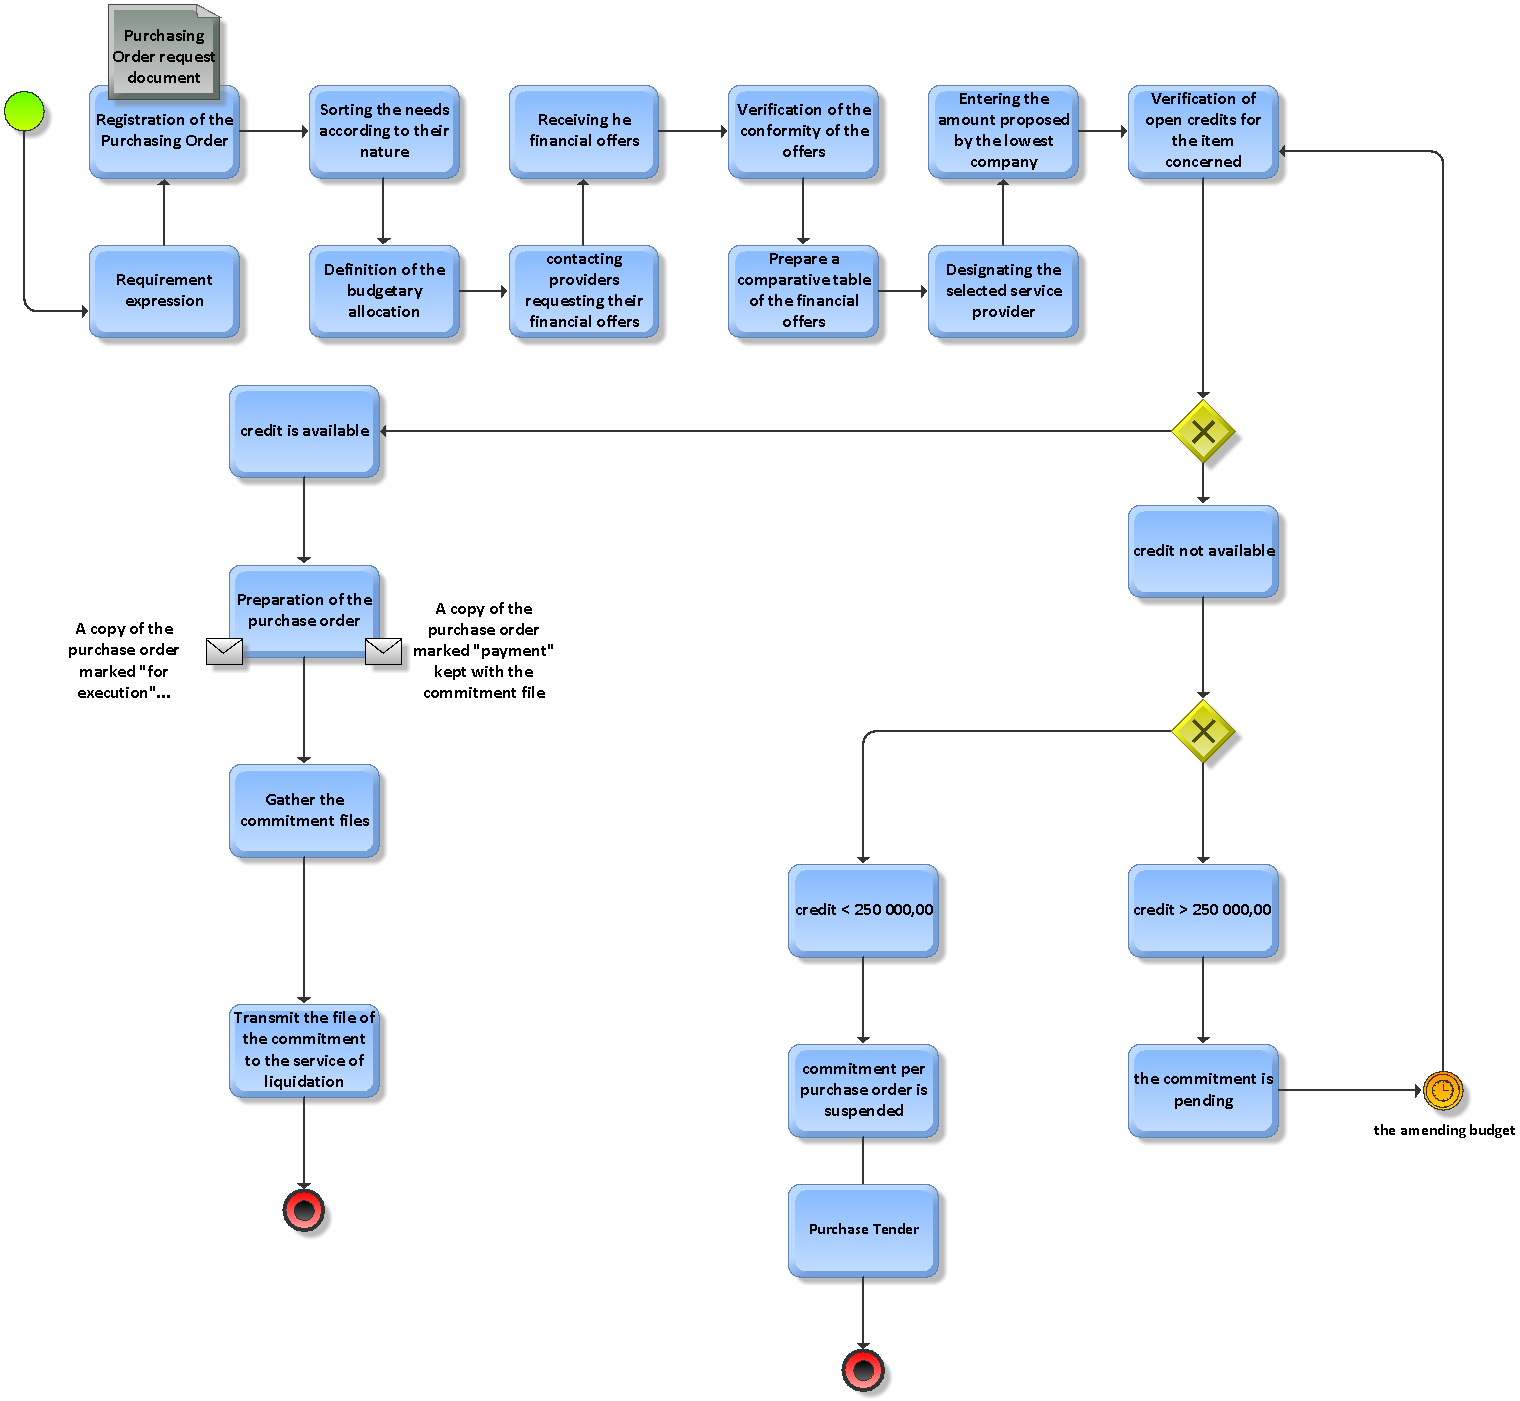
\includegraphics[scale=.3]{bpmn}
\caption{BPMN representation of the purchasing business process}
\label{bpmn_model}
\end{figure}
\clearpage

\section{Limitations of the current purchasing business process and challenging motivations}
\subsection{Motivation scenario}
\par In this motivation scenario, we consider purchasing order in a computer science department. Purchasing order in this scenario expresses the  need for a powerful computer to run heavy AI calculations. Here, we will not describe the execution of the entire purchasing business process. We will focus on three steps: "requirements expression, ” ”"purchasing order registration," and "designating the selected service provider" (figure \ref{bpmn_model}). Processing in these steps constitutes the core of our proposition.
\par Professor X is beginning a project on the implementation machine learning technique on big data. He identified the need for a new laptop workstation with the following technical features:
\begin{itemize}
\item Graphics (GPU): NVIDIA GTX 1050 GPU with 4GB RAM
\item Processing (CPU): 2.8GHz Intel Core i7-7700HQ
\item RAM: 32GB 2400MHz DDR4 RAM 
\item Storage: 1TB SSD
\end{itemize}

\par A purchasing order of two Dell XPS 15 9560 laptops is established and communicated to the department head. Purchase order was then sent to the three vendors to receive financial offers. \textbf{Vendor A}, \textbf{Vendor B},\textbf{Vendor C}, responds, respectively, with 1750\$, 1.800\$ and 1910\$ . Purchasing order finds its way through the purchasing business process, and \textbf{Vendor A} will be selected as it is the lowest bidder.


\par In fact, even if \textbf{Vendor A} has the lowest financial proposition, the proposed price exceeds average price of the same product in Amazon by 250\$. The actual business process does not cover this use case for two reasons: first, the lowest bidder rule, and, second, the absence of a formal mechanism to assess how reasonable the prices are. 

\par In addition to the financial side, quality of purchased reference is not assessed. Moreover, possible technical problems and failures that may occur after some time of use have not been verified. In this case, an alternative product with minor differences from the initial requirements may be proposed. Finally, from an optimization perspective, the purchasing business process does not involve checking the local IT equipment stock to identify computers that meet approximately the initial criterion and requires only a maintenance effort.

\subsection{Diagnosis of the current challenges}
\par To diagnose the current limitations and position our proposition, we will take a fragment of the purchasing business process BPMN model figure \ref{giagnostic}:

\begin{figure}[H]
\centering
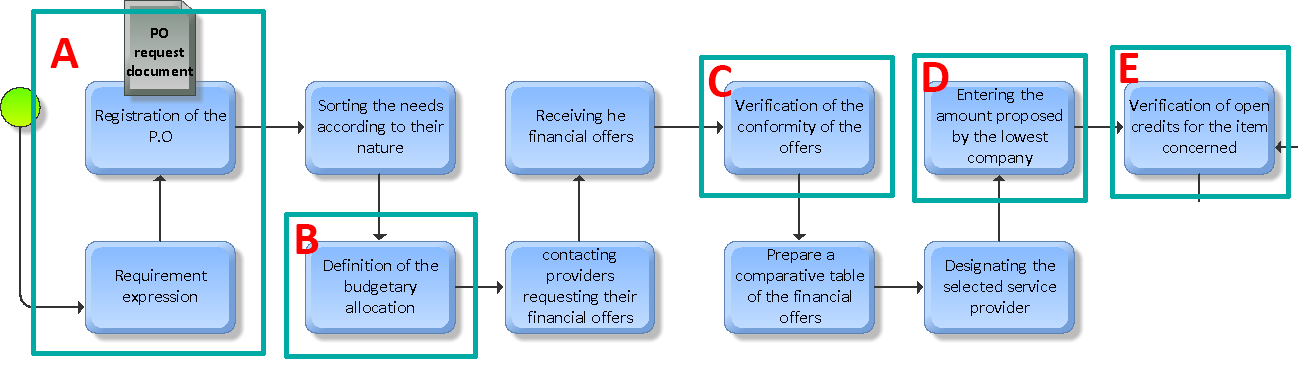
\includegraphics[scale=.3]{giagnostic}
\caption{Diagnosis of current challenges in the current purchasing business process}
\label{giagnostic}
\end{figure}

\begin{enumerate}[A.]
\item The user expresses the needs through technical specifications without any visibility about the future material and the expected budget compared with the market. Conversely, the user cannot consult the available products in the local IT equipment stock of the university. 
\item Budgetary allocation is defined without a clear visibility about the actual prices in the market.
\item The verification of conformity is done comparing to initial requirements without consulting a formal technical repository for validation, and the preparation
\item The lowest bidder is selected. And as previously stated, his offer is a good deal technically and financially. 
\item Verification of the open credit is done after consultation with vendors. If the open credit is not sufficient, the purchasing order is blocked or reported while we have gone through several step and spends considerable time.
\end{enumerate}
\subsection{Positioning of the proposed solution}

\begin{figure}[H]
\centering
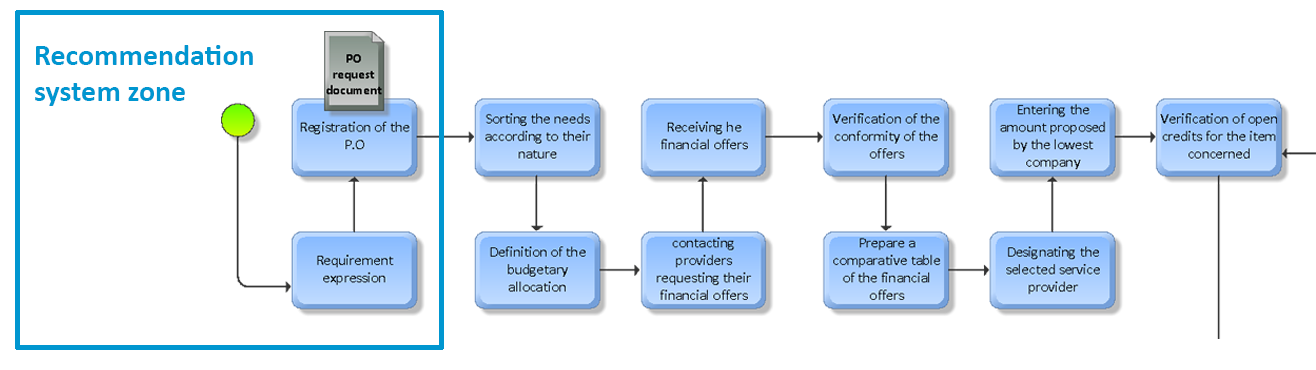
\includegraphics[scale=.3]{zone}
\caption{Recommendation system operating zone}
\label{zone_figure}
\end{figure}

\par Figure \ref{zone_figure} shows that the recommendation system operates at the beginning of the process when the user expresses the initial requirements. Its role is to establish an optimal purchasing order. The recommendation system aims to overcome challenges A, B, C, D, and E, as follows:
\begin{enumerate}[A.]
\item The recommendation system provides the user with accurate and updated information on the future product. These information concerns the technical characteristics and reviews representing previous user's feedback. Moreover, the recommendation system proposes the available products on local storage to check if a matching product exists.
\item The recommendation system provides the user with the actual market prices. Defined budgetary allocation should be reasonable and close to market costs.
\item The recommendation system verifies conformity according to initial requirements and propose alternative products by consulting online e-commerce data for technical characteristics and products reviews.
\item The recommendation system enhances the “lowest bidder”-based decision making using a new feature. In addition to proposing the lowest offer, lowest bidder is also evaluated -- in an objective and independent way -- comparing to the market offer in terms of technical specifications and cost. 
\item As the recommendation system provides the user with actual market prices, the user can verify budgetary allocation according to open credit without waiting for vendors’ offers. This approach adds another layer of transparency as the vendors must align to the user budgetary allocation and not the opposite. 
\end{enumerate}
\section{Theoretical background}
\subsection{Process optimization}
\par Business process optimization is the improvement of business processes using prespecified performance measures. These measures represent optimization objectives \citep{ tsakalidis2017towards}.  Business process optimization aims to redesign business processes and generate various instances based on the same initial process specification. These instances were then assessed according to prespecified performance measures. Given its organizational aspect, the implementation of business process optimization is a managerial act. However, it involves technological and technical engineering to meet automation needs. Generally, there is a need for a wider use of information and communications technology (ICT) in business process contexts, especially decision support systems based on artificial intelligence and expert systems \citep{gunasekaran2002modelling}. ICT can support business process optimization as an automation tool, as stated before and through simulation and modeling tools and standards to represent and optimize the design of the business process.
\par Our current research work fits in this perspective using artificial intelligence as a decision support and PBMN models to design and optimize the purchasing business process.

\subsection{Utility theory in artificial intelligence}
\par Utility theory studies and theorizes the choices of individuals and their decision-making process based on initial preferences. Utility here reflects a subjective conception of opinion quality and goodness compared to other options.  Standard neoclassical economic theory describes utility as a set of internally consistent assumptions about options to maximize utility \citep{ fishburn1968utility}. Utility theory has been leveraged as one of the most dominant theories in economics, underpinning rational choice and game theory.
\par Utility theory is an essential element of artificial intelligence. Artificial intelligence is the design of artificial agents that perceive their environment and make decisions to maximize the chances of achieving a goal \citep{gabriel2020artificial}. Hence, AI-based systems involve a utility function that must be maximized by a rational agent.
\par In our proposition, the intelligent recommendation system aims to mimic human behavior by maximizing a purchasing utility function. 
 
\subsection{COBIT 2019}

\par Information Technology Governance (ITG) can be defined as the system by which current and future use of IT is directed and controlled \citep{calder2008iso}. ITG involves evaluating and directing IT use to support the organization and monitoring this use to achieve plans and includes the strategy and policies for using IT within an organization. ITG and its frameworks provide managers with the structures considered necessary to facilitate IT services for academic and business processes \citep{tawafak2020governance}.

\par The overall aim of ITG is to purify business processes and provide justifiable road map to organization strategies. COBIT 2019 \citep{information2018cobit} is an ITG framework intended for this purpose. The first principle of COBIT is that all IT-related activities should support the generation of value for the enterprise. The COBIT 2019 core model in figure \ref{cobit} illustrates that the five domains covered by the COBIT 2019 code model are \citep{cobitdesignguide2019}:

\begin{itemize}
\item Direct and Monitor (EDM): governing body evaluates strategic options, directs senior management on the chosen strategic options, and monitors the achievement of the strategy.
\item Align, Plan, and Organize (APO): addresses the overall organization, strategy and supporting activities for IT
\item Build, Acquire, and Implement (BAI): treats the definition, acquisition and implementation of IT solutions and their integration in business processes.
\item Deliver, Service, and Support (DSS): addresses the operational delivery and support of IT services, including security.
\item Monitor, Evaluate, and Assess (MEA): addresses performance monitoring and conformance of IT with internal performance targets, internal control objectives, and external requirements.
\end{itemize}

\begin{figure}[H]
\centering
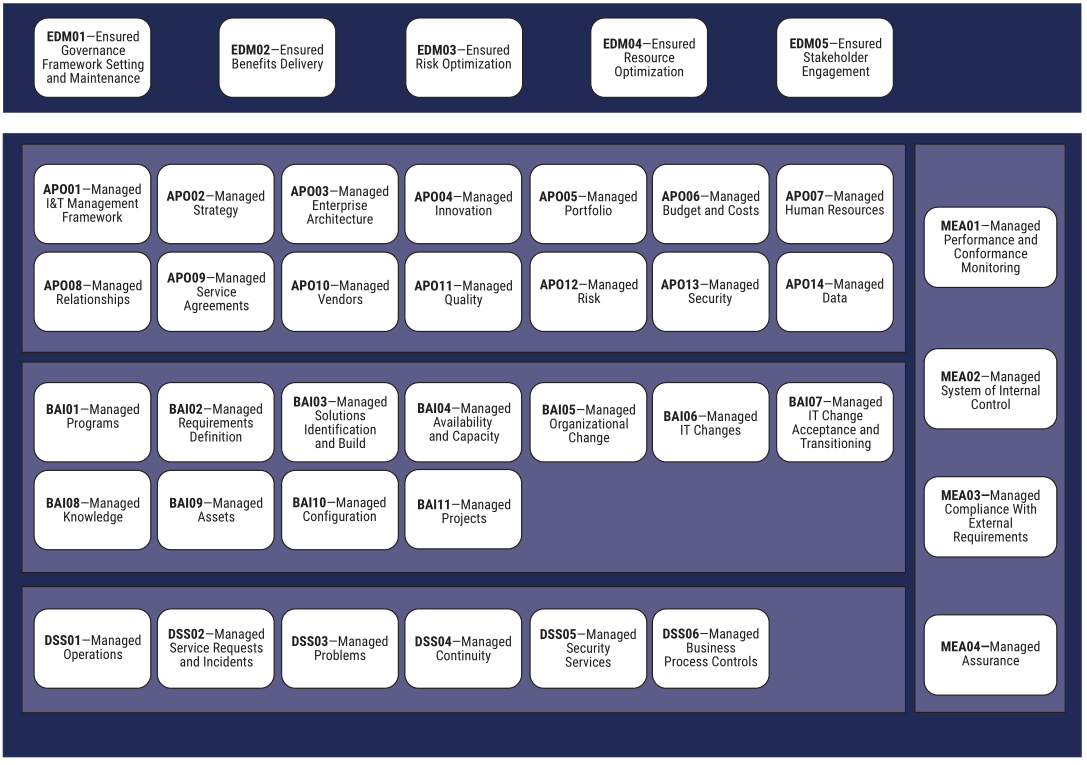
\includegraphics[scale=.5]{cobit}
\caption{COBIT 2019 code model}
\label{cobit}
\end{figure}

\par Our research work fits in the first domain (APO) and uses more GMO which are in direct relation of this paper purpose these two GMO are:

\begin{itemize}
\item APO06 (Budget and Cost Management): Foster a partnership between IT and enterprise stakeholders to enable the effective and efficient use of IT-related resources and provide transparency and accountability of the cost and business value of solutions and services. Enable the enterprise to make informed decisions on the use of IT solutions and services.
\item APO10 (Managed Vendors): Optimize available IT capabilities to support the IT strategy and road map, minimize risk associated with nonperforming or noncompliant vendors, and ensure competitive pricing.
\end{itemize}

\par For each guideline suggested by APO06 and APO10, recommendations are translated into the proposed recommendation system as follows:

\begin{itemize}
    \item APO06.01 Manage finance and accounting: The recommendation system proposed offers a transparent context to manage and account for IT-related costs. Moreover, it offers a visibility on the future investments through the purchasing orders and their impact on the financial systems and accounts. 
    \item APO06.02 Prioritize resource allocation: The recommendation system implements a decision-making workflow that favors prioritizing the recycling and reuse of resources (local database) but also considers the recourse to external actors.
    \item APO06.04 Model and allocate costs : The cost is modeled based on the utility theory. Hence the decision-making process enables the analysis and benchmarking of the allocated cost.
    \item APO06.05 Manage costs: The recommendation system enables the user to explore similar and alternatives products (SOM analysis) to guarantee a certain level of quality while respecting budget. In fact, this approach allows the user to monitor the costs and adjust withing the purchasing order. 
    \item APO10.02 Select vendors : The recommendation system provides the user with reliable and realistic costs. This costs much the average prices in the market for a given product. Based on this information, vendor choice could be done in a pragmatic and transparent way.
\end{itemize}


\section{Design of the intelligent recommendation system }
\subsection{BPMN workflow of the recommendation system} 

\begin{figure}[H]
\centering
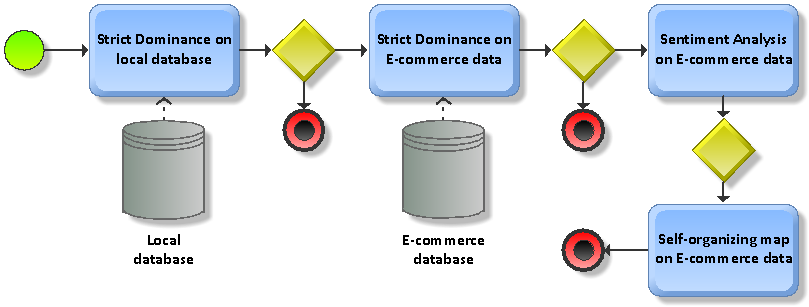
\includegraphics[scale=.5]{rs_workflow}
\caption{workflow of the recommendation system}
\label{rs_workflow}
\end{figure}

\par The workflow in figure \ref{rs_workflow} illustrated in this BPMN model presents the filtering process executed by the recommendation system:
\begin{enumerate}
\item The workflow is triggered when the user provides the initial requirements. 
\item Based on the initial requirements, a strict dominance filtering is performed on a local database. The resulting products are presented to the user, and if the user is satisfied, the workflow is aborted. Otherwise, the user moves to Step 3.
\item Based on the initial requirements, E-commerce data are crawled, and a strict dominance filtering is performed this time on scraped data. The resulting products are presented to the user, and if the user is satisfied, the workflow. Otherwise, the user moves to Step 4.
\item The E-commerce data are subject to a sentiment analysis to reclassify them based on users’ reviews, and the resulting products are presented to the user. If the user is satisfied, the workflow is aborted. Otherwise, the user moves to Step 5.
\item The resulting products from step 4 are processed by self-organizing map classifier and provides the user with a matrix to explore the similarities between products to select the suitable product. Finally, the workflow is aborted.
\end{enumerate}
\subsection{UML modeling of the recommendation system}
\subsubsection{UML sequence diagram}
The sequencing of actions to interact with the intelligent recommendation system are illustrated through the sequence diagram in figure \ref{sequencediagram} :
\begin{figure}[H]
\centering
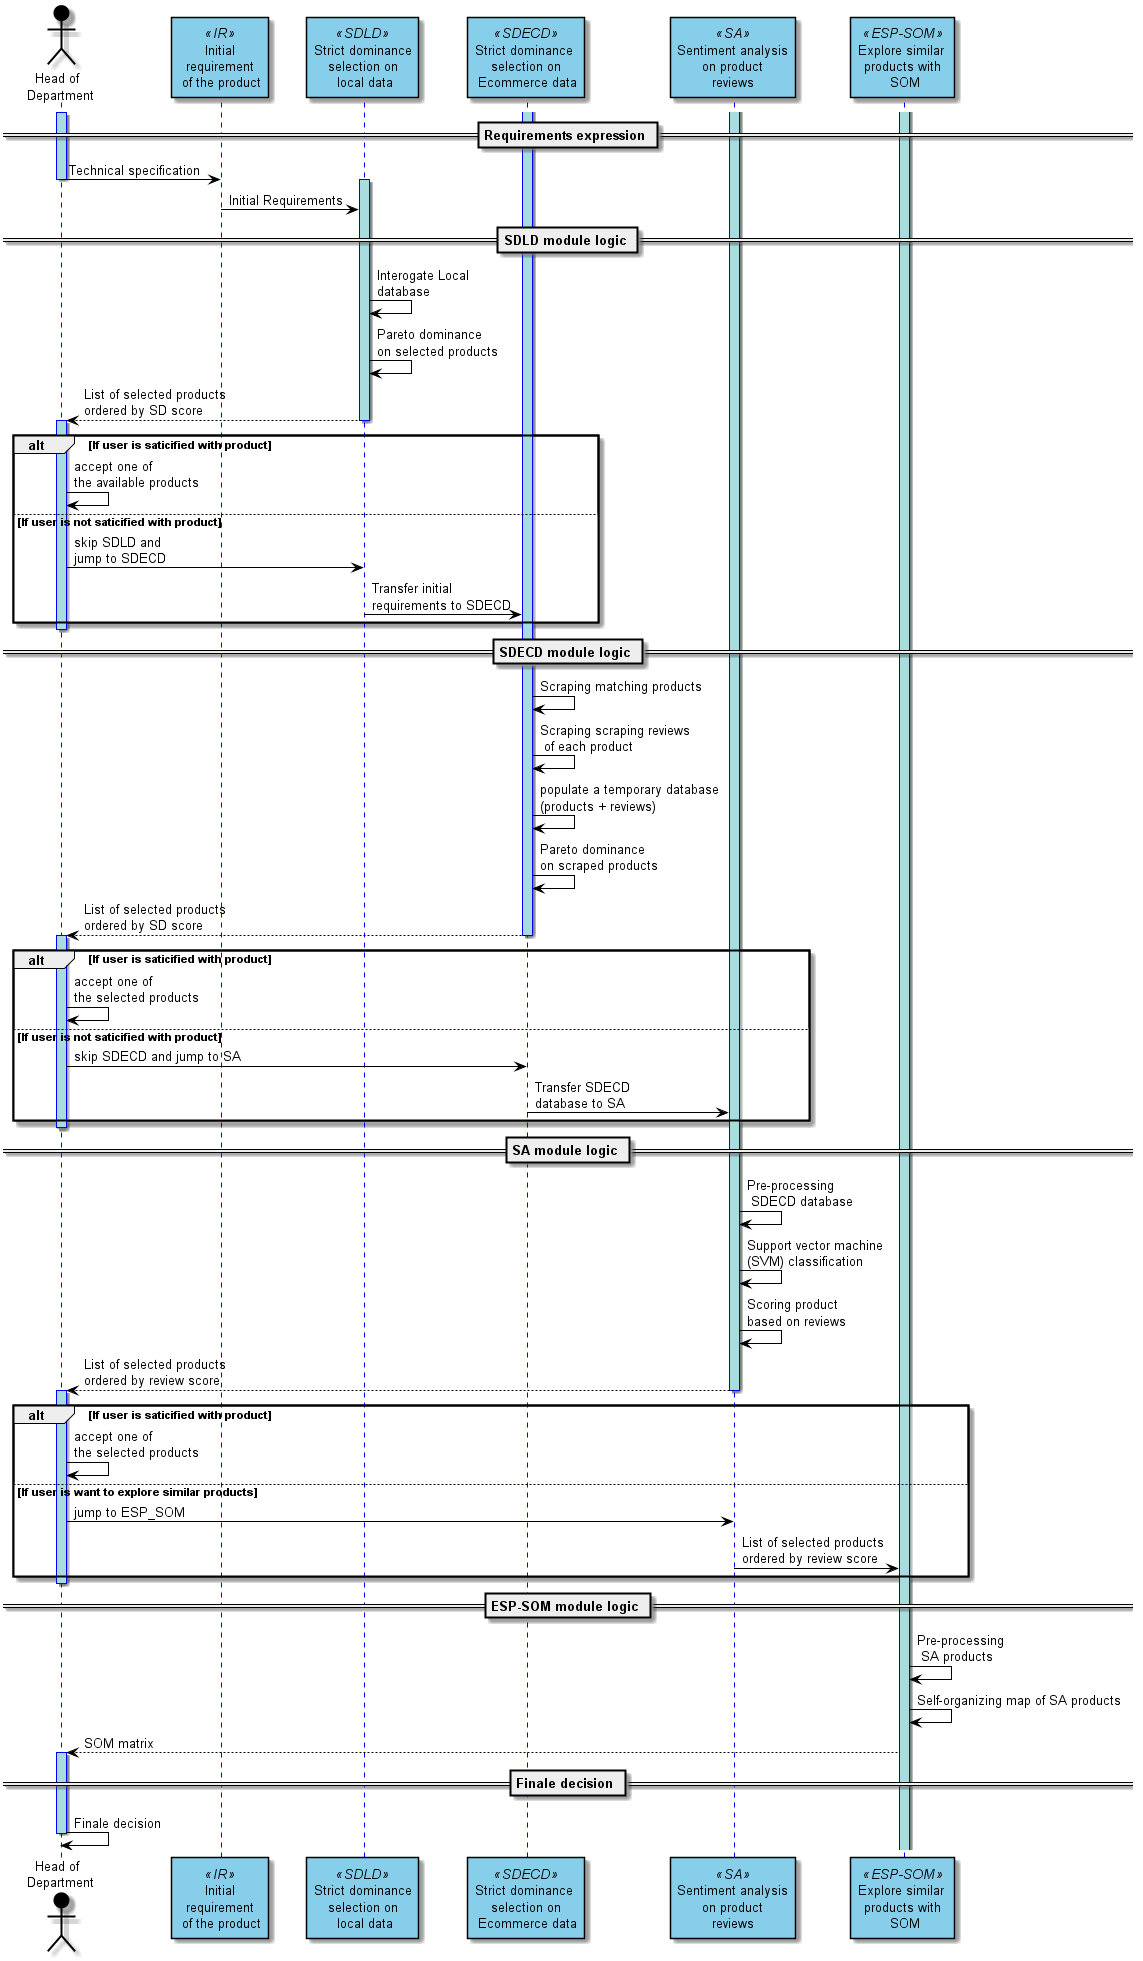
\includegraphics[scale=.30]{sequencediagram}
\caption{Sequence diagram of the Intelligent recommendation system}
\label{sequencediagram}
\end{figure}

\subsubsection{UML component diagram }

The components of the the intelligent recommendation system are illustrated through the component diagram in figure \ref{componentdiagram} :
\begin{figure}[H]
\centering
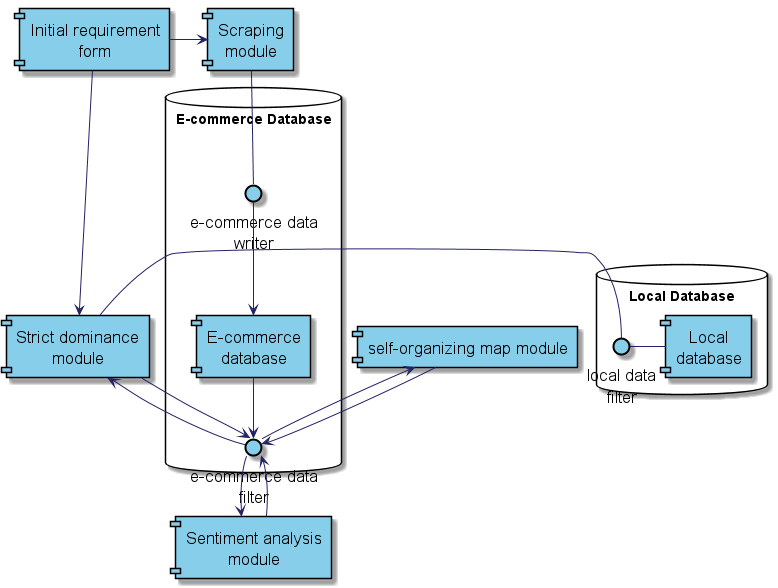
\includegraphics[scale=.5]{componentdiagram}
\caption{Component diagram of the Intelligent recommendation system}
\label{componentdiagram}
\end{figure}

\subsection{System components presentation}
\subsubsection{Initial requirements}
\par Initial requirements represent user preferences expressed as technical features (e.g., Processor generation and RAM capacity …). These purchasing criteria are considered top priority for the final product. For more flexibility and to explore similar products at the end of the process, the entered values of the criteria are allowed a margin of maneuver. For example, the user expresses that minimum RAM capacity is 16 GB, which allows the recommendation system to propose a product with RAM higher then 16Gb and balancing with other technical features.
\subsubsection{Strict dominance module}
\par This module performs data refinement and selection using the strict dominance concept in game theory. This module primarily aims to calculate a strict dominance score for each product given as input and then classify them based on this score. In the recommendation process, we call this module twice, first to classify products issued from the local database and then to classify products issued from scraped data from the e-commerce website. In both cases, this module selects products based on the initial requirements. The products are then refined using strict dominance logic. 

\par In game theory, a strategy is considered strictly dominant when it is better than all other strategies. By contrast, a strategy is strictly dominated when all other strategies are better \citep {straffin1993game}. In our proposition, we use the notion of dominance to calculate a dominance score for classifying our products. This means that products with lower values for all attributes than all others will be given a low score and vice versa. Essentially, strict dominance is used to narrow down the field of choice for real candidates.

\par To implement the concept of strict dominance, we relied on pareto dominance algorithm. Pareto dominance enables the comparison of candidates based on two or more criteria and provides a proper candidate optimal scheme for decision makers \citep {zhang2018pareto}. 

\par Let Up be the utility functions of the product. The utility function Up represents the preferences between products based on criteria p pertaining to the preference set P: 
\par A product X is dominated by product Y if the two following conditions are satisfied:
\begin{itemize}
\item Y is better than X in every criterion, meaning $\forall p \in P, \quad  Up(X) \geq Up(Y)$
\item a product is considered pareto-optimal if it is not dominated by any other product in the selected list.
\end{itemize}

\subsubsection{Local database}
\par This database constitutes an inventory of the “out of service” IT equipment.  This database centralizes maintenance information and facilitates the follow-up of maintenance processes.

\subsubsection{E-commerce database}
\par This database is filled using web scraping technique \citep{varela2021web} on predefined e-commerce websites. Based on the initial requirements, a URL representing the search pattern was constructed for each e-commerce website.
\par Upstream, we have developed a middle-ware for each website that enable the browsing of its DOM and the extraction of product’s information from its HTML tree. The crawled information is stored in two different tables. First, the technical features of each product are stored in the corresponding table. Subsequently, for every product, a set of rows representing its reviews is created and stored in the corresponding table with reference to its parent product. For sentiment analysis efficiency, only products with more than 10 reviews were selected.
\subsubsection{Sentiment analysis module}
\par In the natural language processing (NLP), sentiment analysis (SA) has become one of the many fields of computational studies \citep{bautin2008international}. Sentiment analysis was used to calculate the appreciation score for each product. The appreciation score was calculated through the categorization of positive and negative customer reviews of the product. The polarization of positive and negative reviews was performed using the mean of the supervised learning model. The model was trained on one of the most reliable and large datasets used in this field, which is an Amazon review dataset.
\par In fact, Amazon is one of the largest e-commerce sites as there are numerous number of reviews that can be seen. We used Amazon product data provided by \citep{ni2019justifying}. Current data include reviews from May 1996 to October 2018. The dataset reviews included ratings, text, helpful votes, product description, category information, price, brand, and image features. The dataset is unlabeled and widely used to analyze users positive and negative sentiments toward products.
\par In our analysis, we have used two subsets of global data: “Electronics” and “Office Products.” The total number of reviews in the principal dataset for these two subsets was 26, 575, 666. In our prototype, we used portions of the "small subsets” offered by \\ citep{ni2019justifying} for experimentation purposes. Hence, total review were used to train the sentiment analysis module is 1,539,947 reviews. A typical JSON object of a review of Amazon product data is illustrated in figure \ref{json}: 

\begin{figure}[H]
\centering
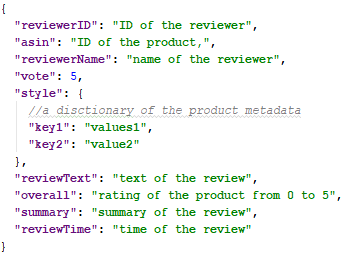
\includegraphics[scale=1]{json}
\caption{Json structure of review object}
\label{json}
\end{figure}


\par To implement the sentiment analysis workflow on our subset, we have adopted the methodologies used in similar works \citep{elli2016amazon}, \citep{xu2015sentiment}, \citep{rain2013sentiment}, \citep{bhatt2015amazon}. The workflow contains four steps (figure \ref{saworkflow}).

\begin{figure}[H]
\centering
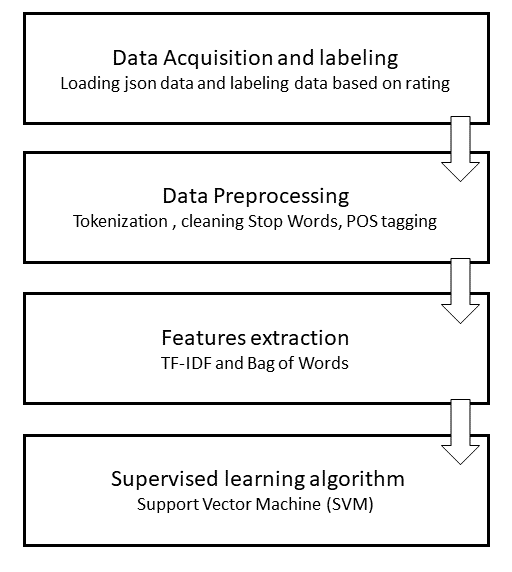
\includegraphics[scale=.5]{saworkflow}
\caption{Sentiment analysis workflow}
\label{saworkflow}
\end{figure}

\begin{itemize}
\item Data acquisition: As stated before, we have acquired our data from 2 subsets, with each subset in the Json format. Regarding the important number of reviews, labelling data manually was very difficult. Hence, data were labeled by an algorithm based on Amazon reviews rating. This rating is represented by a 1 to 5 rating. A rating of 1 or 2 stars is considered negative, while a rating of 4 or 5 is considered positive, 3 stars rating are considered neutral hence not processed in the labeling.

\item Data pre-processing: This step was performed through three stages. First, tokenization, which consists on untying a string sequence into separates entities called tokens. Tokens can be individual words, phrases, and sentences. Second, the Stop Words elimination consists of removing punctuation and all unnecessary text mining strings. This will enhance the accuracy and performance analysis. Finally, the POS tagging helps the model understand the grammatical function of words \citep{pasupa2019thai}.

\item Feature extraction: This step performed through Bag of words and TF-IDF techniques. The bag of word is created from nouns and adjectives selected based on the previous the POS tagging. The bag of word is then used to generates term frequency as text characterization feature. This feature will then be used as input in TF-IDF stage. TF-IDF in turn will weighs the extracted term frequency and also inverse document frequency. TF and IDF scores are then calculated for each word as well as the TF*IDF weight for each word. The value TF*IDF weight determine the rarity of words, lower TF*IDF value means o high frequency of the word. 

\item Support vector machine (SVM): SVM is a machine learning method that has become exceedingly popular for neuro-imaging analysis in recent years. Owing to their relative simplicity and flexibility for addressing a range of classification problems, SVMs distinctively afford balanced predictive performance, even in studies where sample sizes may be limited \citep{pisner2020support}. SVM has also proven its accuracy in sentiment analysis classification especially when trained over the amazon reviews dataset.  In \citep{nasr2017building} and  \citep{ haque2018sentiment} the accuracy of SVM has being demonstrated comparing to other supervised learning algorithm.
\end{itemize}

\subsubsection{SOM analysis module}
\par The Self-Organizing Map (SOM), with its variants, is the most popular artificial neural network algorithm in the unsupervised learning category \citep {kohonen2012self}. It provides topology-preserving mapping from high-dimensional space to map units. Map units or neurons usually form a two-dimensional lattice; thus, mapping is a mapping from a high-dimensional space onto a plane. \citep {kohara2018clustering}. Each unit has a set of weights that are compared to the input data to find the nearest unit (commonly measured with Euclidean distance) to the input data, which is called the best matching unit (BMU). The weights of the BMU and its neighbors were adjusted. At the end of the training phase, A topological map (commonly a 2D map) was established. The topological neighborhood of the units reflects the similarities in the input data that activate them. Figure \ref{som} illustrates the concept of the competitive learning algorithm \citep {kohonen2013essentials}.

\begin{figure}[H]
\centering
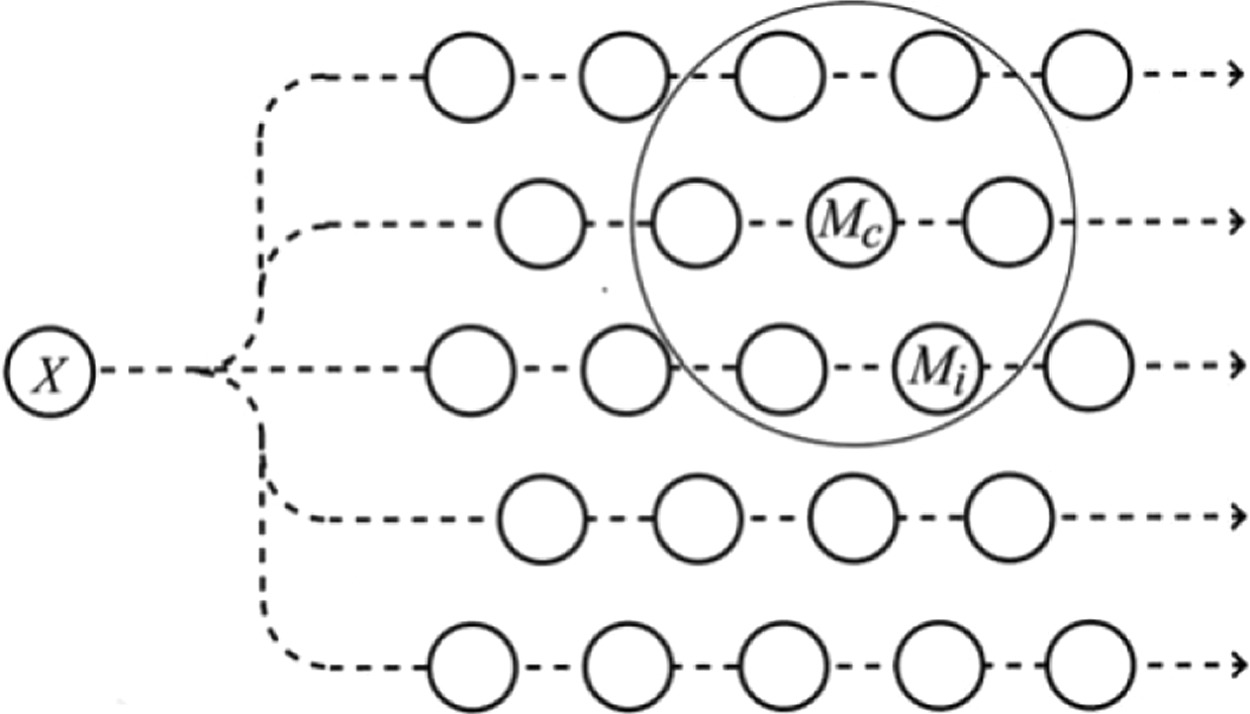
\includegraphics[scale=1]{som}
\caption{Illustration of a self-organizing map. An input data item X is broadcast to a set of models M i , of which M c matches best with X. All models that lie in the neighborhood (larger circle) of M c in the grid match better with X than with the rest \citep{wandeto2017detection}}
\label{som}
\end{figure}

The SOM has been used as a purchase decision-making support in many studies \citep {kohara2006purchase} \citep {martins2017intelligent} \citep {kohara2013selecting} \citep {cho2014clustering}. From this perspective, we use SOM in our recommendation system to provide users with more purchasing options by exploring new opportunities. In fact, at the end of sentiment analysis of primary data, the user has a first classification of selected products based on technical features and review score. The purchasing order can then be established based on this classification. Otherwise, the user can have a deeper discrimination of the classification by discovering similarities between the selected products using SOM analysis. For example, the product X rank is 5/10; however, in the SOM 2D grid, this product is located near product A, which ranks 1/10 and is located in the same cluster. Hence, the choice of Product X may present a potential benefit.


\section{Implementation of the simulation scenario}
\subsection{Presentation of the simulation data}
\par Implementation scenario of the proposal simulates a purchasing of computers in our computer science department. Simulation data are then composed of   local and e-commerce data.
\subsubsection{Local database}
\par To prepare our demonstration, we did an inventory in our computer science department to list and identify the existing desktop computers and laptops. Using this inventory, we built a local database (figure \ref{localdatabase}) that references the technical specifications of each product and its operating state. Here, we mean, by operating state, whether the product is functional or not. If a product is out of service, the required level of maintenance is identified.
\begin{figure}[H]
\centering
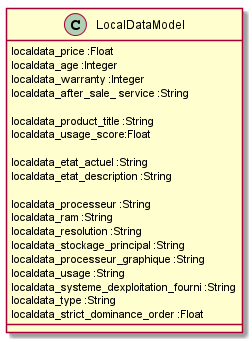
\includegraphics[scale=.7]{localdatabase}
\caption{Local database structure}
\label{localdatabase}
\end{figure}

\subsubsection{E-commerce scraped database}

\par Leveraging data from the web presents both researchers and practitioners with big challenges as well. Apart from the need to learn and deploy new tools and technologies capable of accommodating big data, researchers and practitioners intending to use web scraping in their research projects must comply with a number of legal and ethical requirements \citep{krotov2018legality}. Our scraping module is developed with respect to the following ethical requirements:

\begin{itemize}
\item Terms of Use: Respect to the website we used
\item Purpose of Web Scraping: none profit usage
\item Damage to the Website: respect the time out and amount of data
\item Individual Privacy: we don't scrap any personal information
\item Organizational Privacy and Trade Secrets: we don't scrape o have access to any privacy or thread secrets
\end{itemize}
\subsubsection{Data enhancement}
\par Due to a technical constraint, the reviews of each data are enhanced by external reviews from the amazon review database. In fact, when accessing the detailed page of the product only the first ten products are displayed, and to access other reviews, manual navigation must be performed.




\subsection{Technical specification}

\par The implementation prototype was developed with Django framework. Django is a high-level Python web framework that encourages rapid/clean development and pragmatic design \citep {forcier2008python}. Django is based on the MVC design pattern \citep {leff2001web} and enable a fluent integration with a large number of python libraries. The following table (table \ref{specification}) resume the technical specification and the used libraries.

\begin{table}[H]
\centering
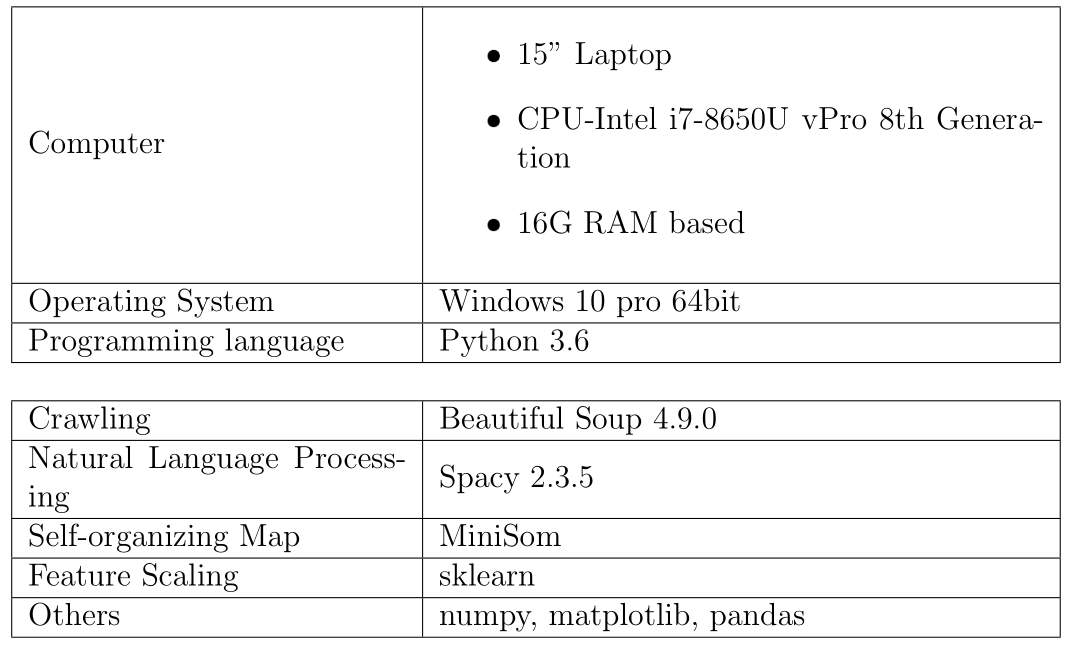
\includegraphics[scale=.4]{specification}
\caption{Technical specification}
\label{specification}
\end{table}

\subsection{Experimental use case}
\subsubsection{Initial requirements}
\par In this step (figure \ref{01_Initial_requirements} ), the user fills the minimum required preferences and the approximate budget allocated. Further information is also provided about the purchasing order, namely the subject, and a short description of the purpose of the future purchasing order. 

\begin{figure}[H]
\centering
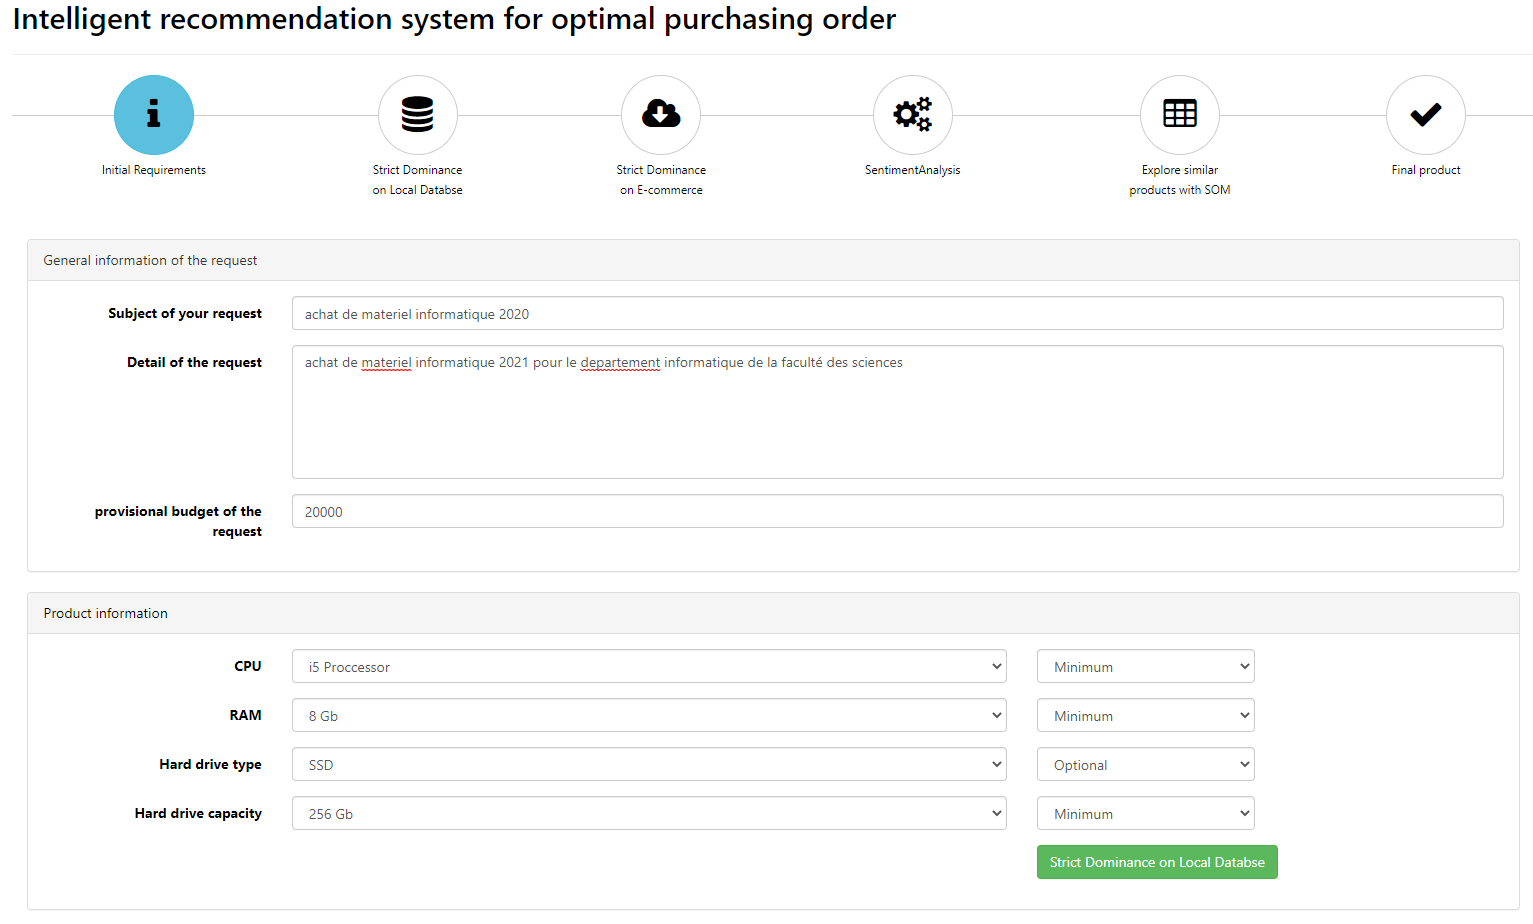
\includegraphics[scale=.3]{01_Initial_requirements}
\caption{Initial Requirements}
\label{01_Initial_requirements}
\end{figure}

\subsubsection{Strict dominance on local database}
\par In this step (figure \ref{02_LocalDatabase}) a selection query is performed based on the initial requirement data entered by the user. Hence, the filter is composed of the desired technical specifications and weighting of each specification. A strict dominance score was then calculated, and the selected products were classified based on this score. The top ten products were then presented to the user.

\begin{figure}[H]
\centering
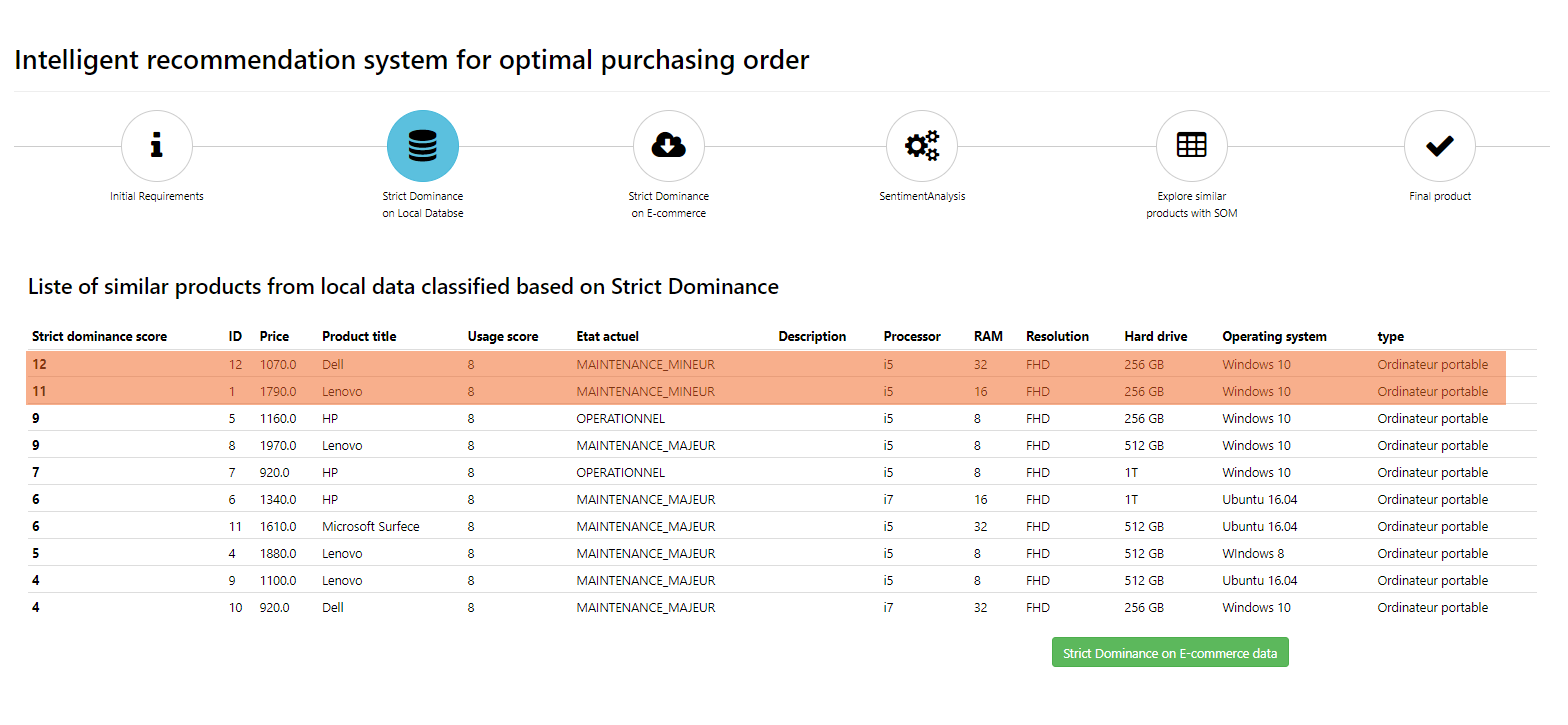
\includegraphics[scale=.3]{02_LocalDatabase}
\caption{Strict Dominance on local database results}
\label{02_LocalDatabase}
\end{figure}

\par If the user is satisfied with the result, he will communicate the product ID to the administration to get the product through a recovery procedure. To browse the other step of the demonstration, we considered that the user would go through all the steps. The next issue is the strict dominance of e-commerce data.

\subsubsection{Strict dominance on e-commerce data}
\par In this step (figure \ref{03_Ecommerce}) the initial requirement data entered by the user are used as entree for a scarping. This scraping module uses technical specifications and their weights to scrape data from an e-commerce website. A strict dominance score was calculated for the selected products from the scraping module.

\begin{figure}[H]
\centering
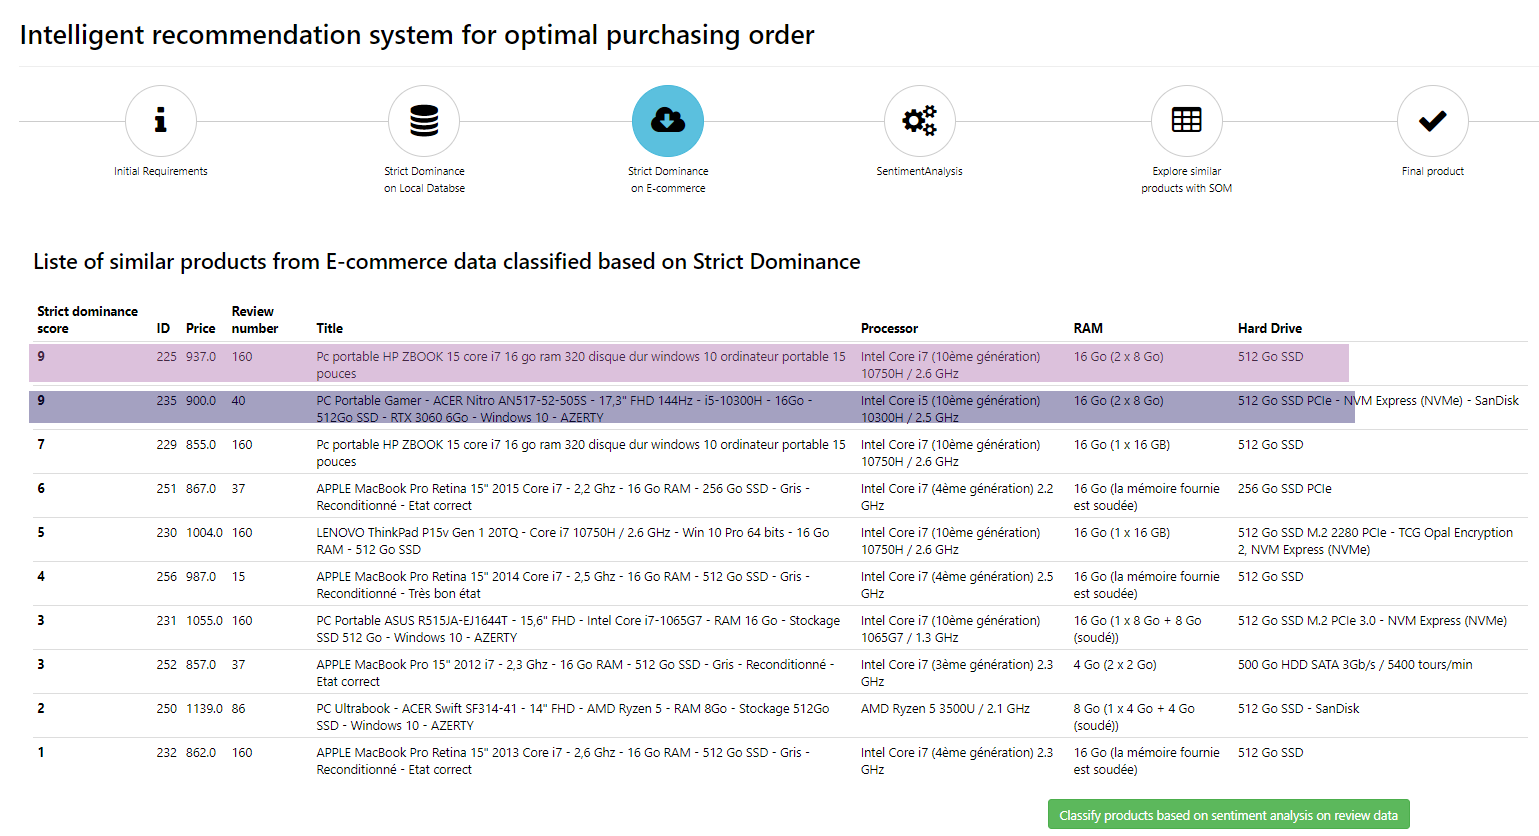
\includegraphics[scale=.3]{03_Ecommerce}
\caption{Strict Dominance on e-commerce data results}
\label{03_Ecommerce}
\end{figure}

\par For each product scraping module import available product reviews and store them to be in the next step.

\subsubsection{Sentiment analysis}

\par For each product the sentiment analysis module perform a NLP on each one
for the previously selected products. This analysis calculates the sentiment analysis score and orders products based on this score.The results of this step are highlighted in figure \ref{04_Sentiment_analysis}.

\begin{figure}[H]
\centering
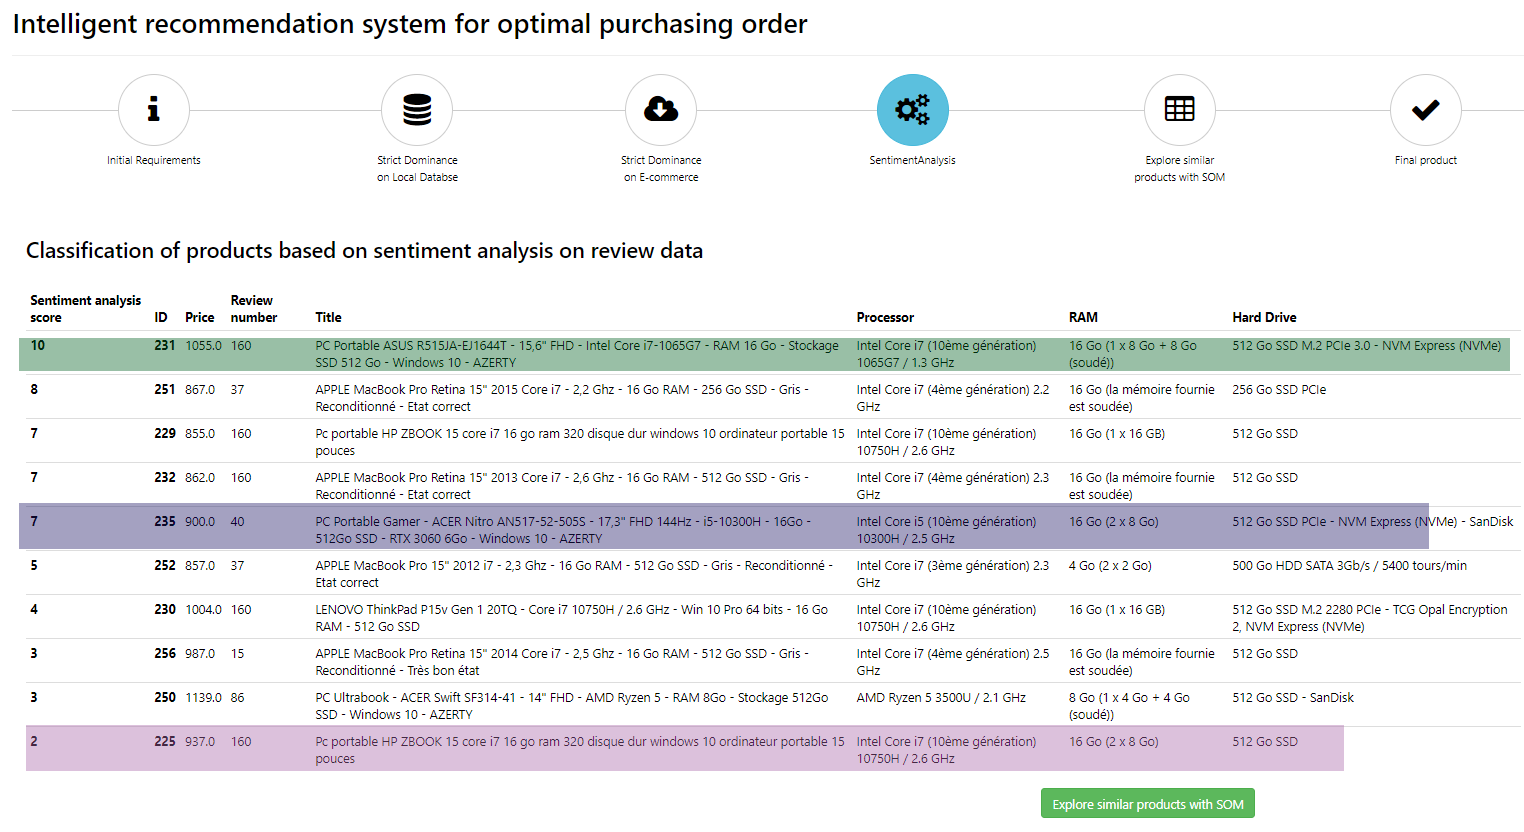
\includegraphics[scale=.3]{04_Sentiment_analysis}
\caption{Sentiment analysis results}
\label{04_Sentiment_analysis}
\end{figure}

\subsubsection{Explore similar products using SOM analysis}

\par In this step (figure \ref{05_SOM}) a SOM map is presented to the user with nods representing products IDs. For each product, the nearby counterparts are more similar than those that are further away. This enables the user to explore similar products and check more details each time by entering the ID of the product in the appropriate form.

\begin{figure}[H]
\centering
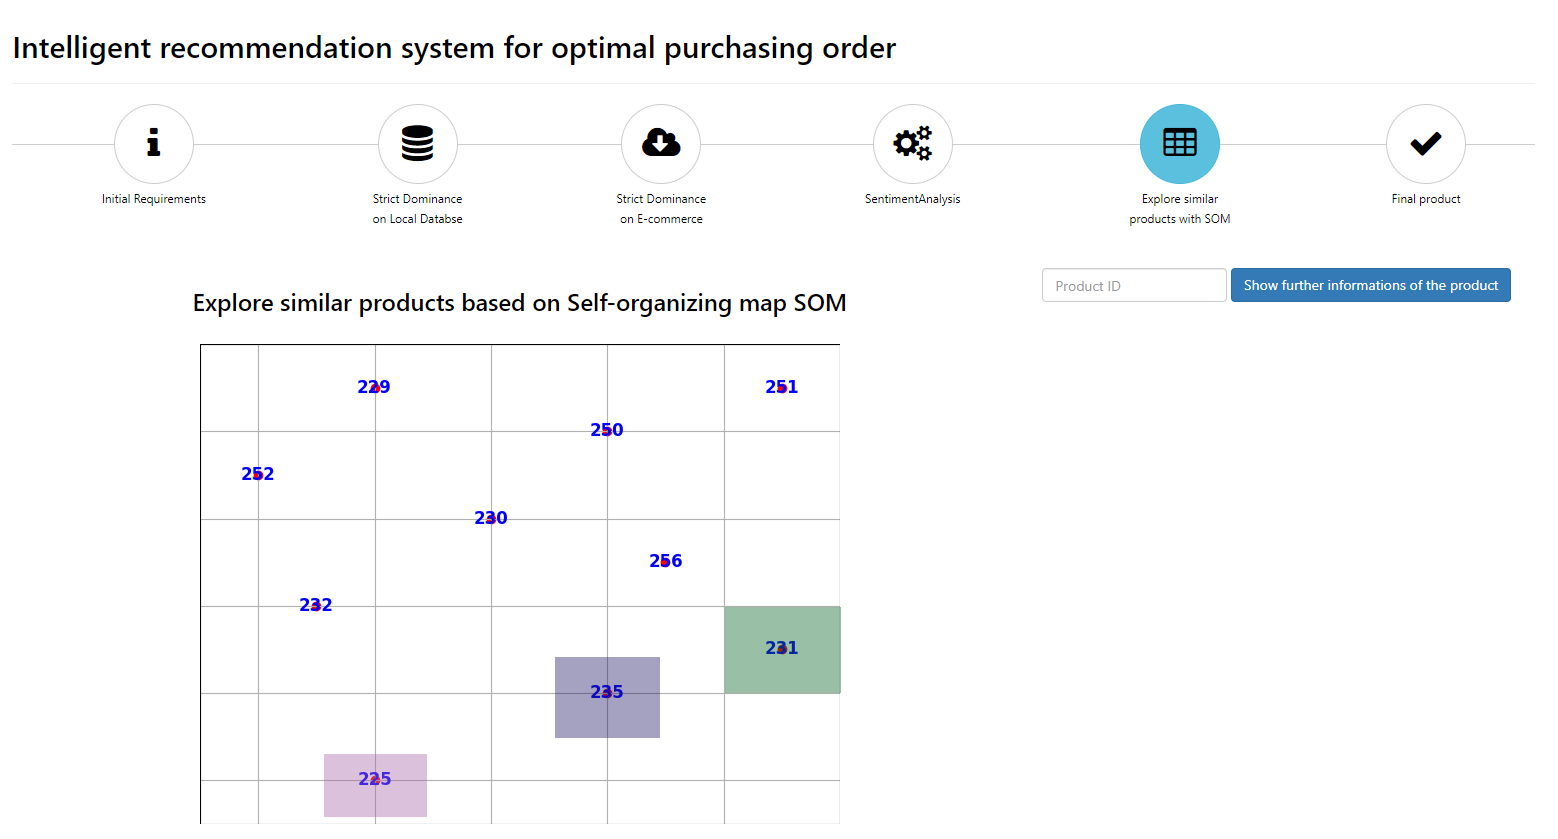
\includegraphics[scale=.3]{05_SOM}
\caption{ SOM map of the selected products from sentiment analysis step}
\label{05_SOM}
\end{figure}


\subsubsection{Final product}

\par The final product selected by the user ( figure \ref{06_Final_product} ). In the next section, the process leading to this choice is explored and discussed.

\begin{figure}[H]
\centering
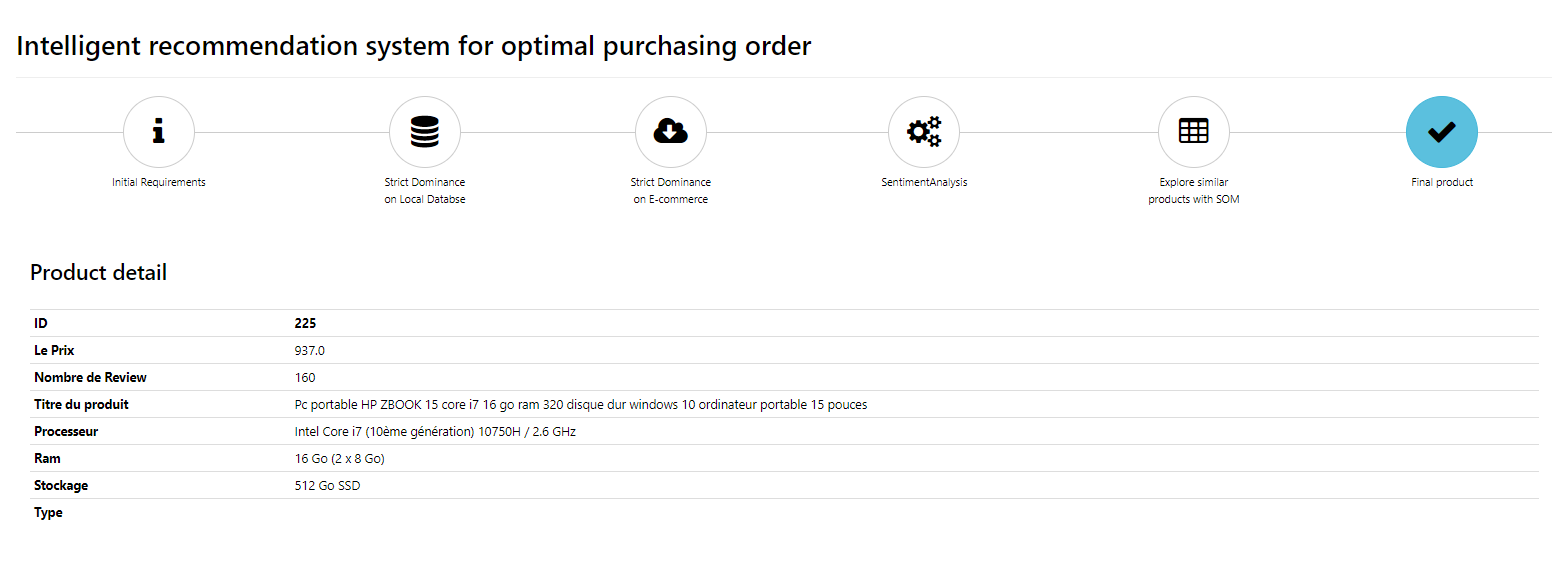
\includegraphics[scale=.3]{06_Final_product}
\caption{Final product information}
\label{06_Final_product}
\end{figure}

\section{Results and discussion}

\par To analyze the efficacy of our intelligent recommendation system, we simulated a recommendation request of the computer science head department above. The recommendation system involves efficient laptops for developing new internal applications. We discuss the execution and results of each step of the recommendation process:
\subsection{Initial requirements}
\par The initial requirements entered by the user are:

\begin{table}[H]
\centering
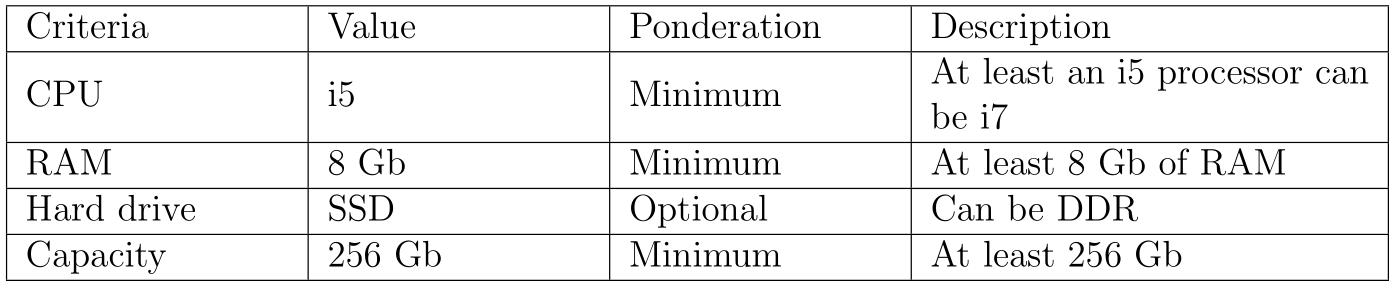
\includegraphics[scale=.4]{res_initail_req}
\caption{Initial requirements}
\label{res_initail_req}
\end{table}

\subsection{Strict dominance on local database}
\par When performing the strict dominance on local data, the algorithm favors products with miner
maintenance with respect to the i5 minimum processor value and maximizing the RAM value.
The weighting of the price is neutralized because the products are already purchased and available internally. The top-scoring products are Product 12 and Product 1 of the database.

\subsection{Strict dominance on E-commerce data}
\par The scraped data are then object to a strict dominance processing, as demonstrated before the algorithm give a score of 9 to products 225 and 235.Product 225 has an i7 processor and 16 Gb in RAM at a price of 937.0, which seems to be a good deal because it has a good configuration and reasonable price. Product 235 is relatively cheaper than 225, but only for an i5 processor.

\subsection{Sentiment analysis}
\par The sentiment analysis on the scraped product gives a quite different result from the previous one. Remarkably, product 225 descended in ranking with a sentiment analysis score of 2. Product 235 maintained a good ranking with a score of 7. It’s if clear that from a user’s reviews perspective the product 231 is a good deal with a score of 10 extracted from 160 review.

\subsection{Explore similar products using SOM analysis}
\par When exploring SOM map, we can see that the product 225 is relatively far from other products. If we combine this information with sentiment analysis results, we can conclude that product 225 represents a good deal in terms of technical specification and user’s reviews. We can also notice that products 235 and 232 are the closest to 225, which means that they are a potential choice, especially 235, which was recommended by strict dominance.

\section{Conclusion and perspectives}
\par As initially stated in this paper, the main goal of the current research work relies in the optimization of the purchasing business process in Moroccan public university in terms of transparency and budgetary optimization.  To achieve this goal, we used a functional-technical approach leading to the development of an intelligent recommendation system that supports the choice of optimal IT equipment for decision makers. All this, in total alignment with Moroccan normative laws, and with COBIT’s guidelines in information system governance.

\par The recommendation system proposes a technical solution based on three concepts: the first one is the strict dominance which belong to utility theory, the second and third belong to artificial intelligence world and are, respectively, sentiment analysis and self-organizing maps. Beyond this technical aspect, we proposed a PBMN model for purchasing business processes. We plan to extend this model to all the business processes of our university to implement a global business process repository. We also used COBIT as an organizational reference to implement the recommendation system with respect to COBIT's guidelines.

\par Moreover, the purchasing process of computer equipment is in constant height demand and must follow the technical evolution while providing the possibility to reuse available equipment in stock and those out of service.


\par Hence, the major contribution proposed in the current paper can be summarized as follows:

\begin{itemize}
    \item The modeling of business processes in public university is established using BPMN in accordance with official regulations. The set of BPMN models constitute a powerful repository for business process execution but also for further optimization.
    \item Governance generally aims to reduce budgetary wastes, and our recommendation system demonstrates a technical and methodological approach enabling this feature.
    \item Implementation of artificial intelligence techniques can bring great value in terms of transparency and fluidity in purchasing business process execution
\end{itemize}


\par Potential limitations can be considered as business limitations and technical limitations:
  
\begin{itemize}
    \item Business limitations: First, the proposed system was modeled to handle one type products, which are computer-related equipment. Hence, we intend to extends our model to other type of products in future works. Conversely, the system proposes optimal purchasing order and assumes that decision makers will rely on this optimal purchasing order to choose between offers. In fact, as perspective, we plan to work on a complete automation of the workflow to also include vendors selection and offers validation.

    \item Technical limitations: NLP is a widely used sentiment analysis technique that enabled us to validate our proposed system. Even working on samples of datasets, we noticed NLP dependency on huge computing power. We intend to experiment with learning and knowledge-based sentiment analysis and assess its computing power consumption and its accuracy compared to NLP. Another technical limitation is related to the web scraping technique, in fact, the users’ reviews are crucial for our system. To guarantee timeliness and reliable reviews, the system has to look automatically in websites, which confront us with the limitations of the web scraping like the permanent changing of website structure and scraping restrictions.
\end{itemize}

\bibliographystyle{agsm}
\bibliography{references}
\end{document}
